Although this is called the intro, I've also but in bits that I want to put in that are general for more than one chapter. These are just bullet pointed \emph{aide memoirs} at the moment but will obviously be fleshed out in time.

\section{Statistical Ecology}

Some general remarks about stat ecol perhaps.

%\section{Themes}
%
%Some sort of general intro here.
%
%\bi
%	\item Morphing
%	\item Modifying penalties
%	\item Computational efficiency
%	\item Realistic physical models!!!!!!
%\ei


\section{Some notational conventions}


\section{Generalized Additive Models}

General GAM setup. The is will mostly be taken from \cite{simonbook}, \cite{rwc} and \cite{marraradice2010}.

\bi
\item Splines
\item objective function
\label{GAMobjfcn}
\item penalties
\label{GAMpenalties}
\item bases - TPRS (and maybe P-splines?)
\label{GAMtprs}
\label{GAMtprspenalty}
\item tensor products
\label{GAMtensor}
\item fitting - GCV REML etc
\label{GAMGCV}
% see p. 122 RWC here GCV vs REML -> same MSE but different tradeoffs in Var and Bias
\item other stuff - MSE, EDF etc
\item \texttt{mgcv}
%	\bi
%	\item MSE
%	Mean squared error is... (look at HTF)
%	
%	\begin{equation}
%\text{MSE}(\hat{f}) = \frac{1}{P} \sum_{j=1}^P (\hat{f}(x_j) - z_j)^2,
%\end{equation}
%the mean difference between the model ($\hat{f}$) evaluated at the prediction points ($\{x_j : j=1 \dots P\}$) and the true value of the function ($\{z_j : j=1 \dots P\}$.) This gives the MSE per model, since here many realisations are run, the mean of these over all simulations is taken and the standard error is calculated.
%	\item EDF
%	
%The estimated degrees of freedom gives an measure of the complexity of the model that was fit to the data. The higher the EDF, the more basis functions were used and  the more complex the model.  Since the models used here are penalised, it is the penalty term that controls the overall ``wigglyness'' of the spline and hence the EDF. Although the basis dimension is set in the model, this is just an upper bound, the smoothing penalty suppresses parts of the model. Therefore basis dimension is not a major concern provided that it is not set too low (\cite{simonbook}, p. 161.) 
%
%	\ei
\ei

\section{Finite area smoothing}

\subsection{Overview of finite area smoothing}

Splines are a popular way of performing spatial smoothing in two dimensions. In this context, they are often used to fit smooth functions over a geographical region. A typical application of this is in ecological modelling; a response (be it simply the presence of individuals in a population or concentration of a chemical) is modelled as a function of its spatial coordinates. The estimated function can then be used to perform inference on the population, whether that be an abundance estimate, density map or a more sophisticated inferential goal. Finite area smoothing simply specifies that the domain over which this smoothing takes place is bounded.

When the geographical region has a \emph{complex boundary}, features from one part of the domain can unduly influence other parts. Considering the boundary as a polygon, a complex boundary is a non-convex polygon, in particular when the non-convexity is relatively extreme. Often this consists of having some peninsula-like feature(s) in the domain with notably different observation values on either side of the feature. Given that there is some scientific motivation as to why those parts of the domain should not affect each other, features such as peninsulae give rise to a phenomenon known as \emph{leakage}.

Leakage occurs when a smoother inappropriately links two pats of a domain (\cite{soap}). The phenomenon is problematic since it causes the fitted surface to be mis-estimated; this can then lead to incorrect inference (eg. biased abundance estimates), which is clearly not desirable. Leakage can be seen in \fig{leakage} where the high values in the upper half of the domain leak across the gap to the lower values below and vice versa.

% leakage example 
\begin{figure}
\centering
% trim order l b r t
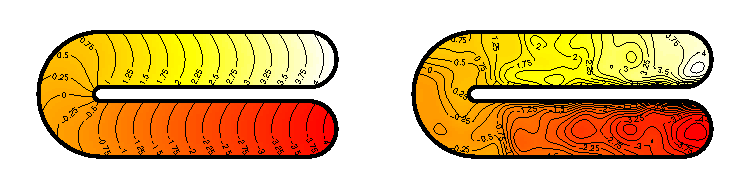
\includegraphics{intro/figs/ramsay-leak.pdf}\\
\caption{An example of leakage. A thin plate regression spline was fit to data sampled from the function on the left, here the model smooths across the gap in the middle of the domain (right.)}
\label{leakage}
\end{figure}

The problem of leakage arises because of the way in which the smoother defines how near objects are to one another. Most smoothing techniques use the Euclidean metric to measure the distance between data. Clearly though, this approach is a flawed: biological populations do not conform to Euclidean geometry in their movement patterns and hence their observed positions will reflect this. Just as whales no not uniformly distribute themselves across sea and glacier, fish do not lay their eggs on land. Natural and man-made barriers carve up the landscape (and seascape), partitioning biological populations; our models should take this into account.

The distribution of the population may be smooth, just not necessarily over $\mathbb{R}^2$ (\cite{wangranalli}). Instead the structure of the domain that is under investigation must be modelled (implicitly or explicitly) for the correct inference to be drawn.

\subsection{Ramsay's horseshoe function as a benchmark for finite area smoothing}

\label{ramsayfunc}

\cite{ramsay} proposes a function which can be used to benchmark new approaches to 2-dimensional smoothing. The function takes the form of a horseshoe shape which is flat across the domain has a gradient along the domain's major axis. This can be seen in \fig{orig-fs}. \cite{soap} modifies the test function by adding curvature across the minor axis of the shape. This was added in order to avoid the horseshoe function lying in the nullspace of their model's penalty, making the problem trivial. It is the second shape that will be used for simulations here and shall be referred to as the \emph{Ramsay horseshoe} throughout; it is shown in \fig{leakage}.

% original horseshoe from Ramsay's paper
\begin{figure}
\centering
% trim order l b r t
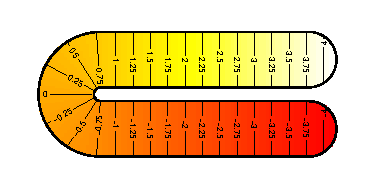
\includegraphics{intro/figs/orig-fs.pdf}\\
\caption{The horseshoe function as it appeared in \cite{ramsay}.}
\label{orig-fs}
\end{figure}

The test function highlights leakage well. As mentioned above, when the smoothing problem is specified in terms of Euclidean distance, the model takes the distance between the points in the two arms of the horseshoe as the distance over the gap in-between them, rather than the distance along the major axis of the shape. This causes the high function values from one side to contaminate the other side (and the low to contaminate the high.) It is easy to see that this causes the smooth to be an inappropriate model.
		
\subsection{Previous approaches to leakage}

The cause of leakage can be characterised in two ways: either the smooth does not respect the boundary of the domain, or the smooth does not take into account the geometry of the domain (in particular with regard to the distance between points within the domain). Previous work in this area has been to combat leakage along these two lines. Work of \cite{ramsay} and \cite{soap} both use a partial differential equation (PDE) boundary condition approach to try to prevent leakage, where as \cite{wangranalli} and \cite{eilerstalk}  attempt to approximate the intrinsic structure of the domain while not treating the boundary as something special in the basis setup. These four main works may be summarised as follows:

\begin{enumerate}
\item \cite{ramsay} proposes finite element $L$-splines (FELSPLINEs). The $L$-spline replaces the usual penalty term (see \secref{GAMpenalties}) with:
\be
\int_\Omega (L_p f)^2 \text{d}\Omega,
\ee
where $\Omega$ is the domain in question and $L_p$ is a roughness operator defined as:
\be
L_p=\Delta^p+c_{p-1}\Delta^{p-1}+\dots+c_1\Delta+c_0I.
\ee
Here $I$ is the identity operator, the $\{c_0,\dots, c_p\}$ are constants and the $\Delta$ is the Laplacian ($\Delta f = f_{xx}+f_{yy}$ in the usual notation). Although any differential operator could, in principle, be used for $L_p$, the Laplacian gives rise to a set of polynomials which are rotation and translation invariant which is clearly sensible given the objective function solution should not depend on the coordinate system used.

In order to find the minimiser of the objective function, Ramsay takes a finite element approach. First he triangulates the domain, then he constructs a set of bivariate quadratic polynomial basis functions over each triangle, specifying that there be continuity over the edges of the triangles. By taking the FELSPLINE objective function and transforming it into a variational form (in the same way as a PDE is), the approximation to the minimiser of the objective function is found. 

Since the triangulation and hence the penalty of the FELSPLINE is only calculated over the domain, and the continuity is specified over neighbouring cells, the method prevents leakage. However, although FELSPLINE does not exhibit leakage on the original horseshoe (as in \fig{orig-fs}), in practice the model makes unrealistic physical assumptions. The boundary conditions of FELSPLINE specify that the gradient is zero, along normals to the boundary. This is not always physically realistic. \cite{soap} show that by using a different response function for the horseshoe shape, the FELSPLINE performance begins to falter.

FELSPLINE does not offer a realistic physical model and is therefore not a viable solution to the finite area smoothing problem in general.

\item \cite{wangranalli} adopt a ``within-area distance'' formulation for thin plate splines. They choose to use the geodesic distance between two points, that being the shortest path within the domain. This gives a definition of how near objects are in the domain. This is then used as the distance in the radial basis functions of a \tprs, rather than using the usual Euclidean distance (see \secref{GAMtprs}).

Wang and Ranalli first create a weighted, undirected graph ($G$, say) with a data point at each vertex and the distance between each pair of vertices as the weights on the edges. They then take the restricted graph of $G$, $G_k$, in which each vertex is only connected to its $k$ nearest neighbours. With this new, restricted graph the geodesic distances between each pair of vertices can be calculated using Floyd's algorithm (\cite{Floyd}).

As the authors point out, the quality of the approximation is dependent on the size of the data set and its density. At low densities the estimated geodesic distance will tend towards the Euclidean, at high densities the approximation tends, asymptotically toward the true geodesic distance (\cite{bernstein}). Even if  dense enough data were available, the method will be rather slow since Floyd's algorithm is cubic in the number of vertices (the size of the data set). Finally, although the $k$-nearest neighbours algorithm used is not specified in the paper, in general such procedures are computationally expensive, adding another source of impedance to the technique.

Taking these points into account, Wang and Ranalli's approach appears cumbersome, slow and dependent on dense data.

\item The soap film smoother (\cite{soap}) uses a rather simple physical model to prevent leakage from occurring. First, consider the domain boundary to be made of wire, then dip this wire into a bucket of soapy water, you will then have (provided it doesn't pop(!)) a soap film in the shape of your boundary. Now consider the wire to lie in the $x-y$ plane and the height of the soap film at a given point to be the functional value of the model. This film is then distorted smoothly by moving it toward the data, while minimising the surface tension in the film. The domain ($\Omega$) is bounded by some polygon with boundary conditions that are either known or estimated by a cyclic spline.

Mathematically, the soap film smoother is constructed by first specifying a set of functions $\rho_k(x,y)$, which are each solutions to the Laplace equation in two dimensions:
\be
\frac{\partial^2\rho}{\partial x^2} + \frac{\partial^2\rho}{\partial y^2} = 0
\ee
except at one of the knots ($x^*_k,y^*_k$). Then, solving Poisson's equation in 2-dimensions:
\be
\frac{\partial^2 g_k}{\partial x^2} + \frac{\partial^2 g_k}{\partial y^2} = \rho
\label{soap-poisson}
\ee
with $\rho=\rho_k(x,y)$, where $k$ indexes the knots and the boundary condition $\rho=0$. The set of basis functions for the soap film smoother, $g_k(x,y)$ is found, along with $a(x,y)$ (the solutions to \eqn{soap-poisson} when $\rho=0$, subject to the boundary condition). These bases are then summed to form:
\be
f(x,y)=a(x,y)+\sum_{k=1}^n \gamma_k g_k(x,y),
\ee
the soap film smoother, where the $\gamma_k$ are parameters to be estimated. The (isotropic) penalty term (\secref{GAMpenalties}) is:
\be
\int_\Omega \Big(\frac{\partial^2 f}{\partial x^2}+\frac{\partial^2 f}{\partial y^2} \Big)^2\text{d}x\text{d}y,
\ee
Differing from the standard \tprs\ penalty since: (\emph{i}) the integration occurs only over $\Omega$, (\emph{ii}) there is no mixed derivative term, and (\emph{iii}) the whole integrand is squared rather than each term individually. This allows the $x$ and $y$ term's derivatives to be traded off against each other so the nullspace of the penalty is infinite dimensional. This allows those functions in the nullspace to be sufficiently wiggly to meet any boundary conditions.

The solution of the PDEs above, yielding the basis and penalty, is the most computationally expensive part of the procedure. Knots to use for $x_k^*$ and $y_k^*$ must be specified, usually using a grid. Numerical problems occur when knots are placed in boundary cells in the PDE solution grid.

Although mathematically elegant, the soap film smoother is a rather complex model. It also treats the boundary differently from the interior and uses a cyclic spline in order to approximate the boundary values. This treatment of the boundary seems rather unnatural and it may not always be physically realistic to consider the boundary in such a way.

\item An alternative approach to treating the boundary as something special is to transform the space in which the points lie to instead lie in a different domain which is more suitable for smoothing. For example, with Ramsay's horseshoe, it seems intuitive to simply bend the horseshoe into a long strip and then smooth on that domain.

Indeed, \cite{eilerstalk} proposed using the \sch\ transform for this very purpose (I, independently, came to the idea in 2008 via BBC Radio 4.) Using the \sch\ transform for smoothing will be elaborated on in chapter \ref{chap-sc}, so only a brief summary is given here.

[[TALK ABOUT CURRIERO HERE!]]

The basic idea is to find a function, $\phi$ say, that takes points in the domain the data lie in ($W$) and maps them to a domain ($W^*$) in which the boundary is less complex ($\phi : W \mapsto W^*$, mathematically).

Creating some kind of mapping between the space in which the data lies and the space in which conventional smoothers perform well is convenient. Not having to setup a new basis structure and relying on long tested methodology is clearly appealing. This approach also benefits from not treating the boundary as a special in the basis setup.
\end{enumerate}

Chapters \ref{chap-sc} and \ref{chap-mds} expand on the ideas in the last method; of using a transformation of space and conventional smoothers to solve the problem of leakage in finite area smoothing.

\section{Distance sampling}

What do I want to say here?

\begin{itemize}
	\item What is DS?
	\item Why and when use it? (and who/how many do)
	\item The detection function - assumptions, current issues
	\item Why mixtures are better.
	\item Death of CDS/MCDS
\end{itemize}

Distance sampling is the name given to a collection of analysis and field study methods which, when put together allow practitioners to assess the density and abundance of biological populations. Distance sampling is an extension of normal quadrat sampling, where an observer counts all of the animals (or plants) in a certain pre-determined area. The difference being that in quadrat sampling the probability of detection within the study area is assumed to be one however, in distance sampling, the probability of detection decreases with distance from the observer. Observations are made from a series of lines which the observer walks down (line transects) or from points dotted around the survey area (point transects) where the observer remains stationary and observes the plants or animals around him/her. The observer records the distance of those individuals seen (or heard) sometimes along with other information (such as size of the individual, sex, weather conditions or habitat type).

\subsection{From density to distance sampling}

Given we wish to estimate the density $\hat{D}$ of some biological population, in general we can write
\begin{equation}
\hat{D} = \frac{n}{a},
\end{equation}
where $n$ is the number of individuals we observe and $a$ is the area in which we observe them. This follows from the definition of density. Say that we use a strip transect survey, in this case we survey $k$ strips, counting all the observed individuals. If each strip is of length $l_i$ such that $\sum_{i=1}^k l_i =L$, the total length and that each strip has some fixed width $2w$, we can then write
\begin{equation}
\hat{D} = \frac{n}{2wL}.
\end{equation}
Now consider the case in which we are not certain that we observe everything in our strips. Then, what we might do is replace the fixed width $w$ with an estimated \textit{effective strip (half)-width}, $\hat{\mu}$. The effective strip width is the point at which we miss as many individuals within a distance of $\hat{\mu}$ from the line, as are observed beyond $\hat{\mu}$. Density can then be expressed as:
\begin{equation}
\hat{D} = \frac{n}{2\hat{\mu}L}.
\end{equation}
Now, how is $\hat{\mu}$ to be estimated? 



In this case we must not only record how many individuals were spotted, but also their distance from the line that we walk.






